\documentclass[12pt]{article}
\usepackage[utf8]{inputenc}
\usepackage{amsmath, amssymb, amsthm}
\usepackage{enumitem}
\usepackage{geometry}
\usepackage{fancyhdr}
\usepackage{pgfplots}
\usepackage{tikz}
\usepackage{float}
\usepackage{graphicx}
\DeclareMathOperator{\Tr}{Tr}
\DeclareMathOperator{\RR}{\mathbb{R}}
\DeclareMathOperator{\rng}{rng}

% Page setup
\setlength{\headheight}{15pt}
\geometry{letterpaper, margin=1in}
\setlength{\parindent}{0pt}
\setlength{\parskip}{1em}
\pagestyle{fancy}
\fancyhf{}
\fancyhead[L]{\textbf{Sebastian Griego}}  % Replace with your name
\fancyhead[C]{\textbf{ODEs}}  % Replace with your course name
\fancyhead[R]{\textbf{Assignment \#3}}  % Replace with your assignment number
\fancyfoot[C]{\thepage}

\newenvironment{problem}[1]{
    \textbf{Problem #1:}
}{
    \rmfamily \vspace{1em}
}

\newenvironment{solution}{
    \textbf{Solution:}
    
}{
    
    \vspace{2em}
}

\begin{document}

\title{Homework \#3}  % Replace with the homework number
\author{Sebastian Griego}  % Replace with your name
\maketitle

\begin{problem}{1}
    Find the general solution of the differential equation \(\vec{x}' = \vec{A}\vec{x}\) for \(A\) given by
    \[
        A_1 =\begin{pmatrix}
            2 & 1 \\
            -1/4 & 1
        \end{pmatrix}, \quad
        A_2 = \begin{pmatrix}
            3 & -1/2 \\
            1/2 & 2
        \end{pmatrix}, \quad
        A_3 = \begin{pmatrix}
            3 & -1 \\
            1 & 1
        \end{pmatrix}
    \]
    Draw the phase diagrams for both the original and transformed systems.
\end{problem}

\begin{solution}
    \textbf{Part 1:} \(A_1 =\begin{pmatrix}
        2 & 1 \\
        -1/4 & 1
    \end{pmatrix}\)

    \(\Tr(A)^2 = 4\det(A)\), so there is only one eigenvalue, \(\lambda = \frac{1}{2}\Tr(A) = \frac{3}{2}\).

    \(A^T \neq \pm A\), so there is only one eigenvector.

    Therefore,
    \[
        \begin{aligned}
            A &= V \begin{pmatrix}
                \lambda & 1 \\
                0 & \lambda
            \end{pmatrix} V^{-1}\\
            \implies \vec{y}(t) &= \begin{pmatrix}
                e^{\lambda t} &te^{\lambda t}\\
                0 & e^{\lambda t}
            \end{pmatrix}\vec{y_0}\\
            \implies \vec{x}(t) &= V \begin{pmatrix}
                e^{\lambda t} & te^{\lambda t} \\
                0 & e^{\lambda t}
            \end{pmatrix} V^{-1} \vec{x}(0)
        \end{aligned}
    \]
    Find the eigenvector:
    \[
        \begin{aligned}
            (A_1 - \lambda I)\vec{v} &= 0\\
            \begin{pmatrix}
                1/2 & 1 \\
                -1/4 & -1/2
            \end{pmatrix} \begin{pmatrix}
                v_1 \\
                v_2
            \end{pmatrix} &= \begin{pmatrix}
                0 \\
                0
            \end{pmatrix}\\
            \implies \frac{v_1}{2} &= -v_2\\
            \implies \vec{v} &= \begin{pmatrix}
                -2 \\
                1
            \end{pmatrix}
        \end{aligned}
    \]
    Find \(\vec{u}\):
    \[
        \begin{aligned}
            (A - \frac{3}{2}I)\vec{u} &= \vec{v}\\
            \begin{pmatrix}
                \frac{1}{2} & 1 \\
                -1/4 & -1/2
            \end{pmatrix} \begin{pmatrix}
                u_1 \\
                u_2
            \end{pmatrix} &= \begin{pmatrix}
                -2 \\
                1
            \end{pmatrix}\\
            \implies \frac{1}{2}u_1 + u_2 &= -2\\
            \implies u_1 + 2u_2 &= -4\\
            u_2 = 0 \implies u_1 &= -4\\
            \implies \vec{u} &=\begin{pmatrix}
                -4 \\
                0
            \end{pmatrix}\\
            \implies V &= \begin{pmatrix}
                -2 & -4 \\
                1 & 0
            \end{pmatrix}
        \end{aligned}
    \]
    Compute \(V^{-1}\):
    \[
        \begin{aligned}
            V^{-1} &= \begin{pmatrix}
                0 & 1 \\
                -1/4 & -1/2
            \end{pmatrix}
        \end{aligned}
    \]
    Jordan decomposition:
    \[
        \begin{aligned}
            A &= V \begin{pmatrix}
                \lambda & 1 \\
                0 & \lambda
            \end{pmatrix} V^{-1}\\
            &= \begin{pmatrix}
                -2 & -4 \\
                1 & 0
            \end{pmatrix} \begin{pmatrix}
                \frac{3}{2} & 1 \\
                0 & \frac{3}{2}
            \end{pmatrix} \begin{pmatrix}
                0 & 1 \\
                -1/4 & -1/2
            \end{pmatrix}
        \end{aligned}
    \]
    Solution for \(\vec{y}\):
    \[
        \vec{y}(t) = \begin{pmatrix}
            e^{\frac{3}{2}t} & te^{\frac{3}{2}t} \\
            0 & e^{\frac{3}{2}t}
        \end{pmatrix} \vec{y_0}
    \]
    Solution for \(\vec{x}\):
    \[
        \vec{x}(t) = \begin{pmatrix}
            -2 & -4 \\
            1 & 0
        \end{pmatrix} \begin{pmatrix}
            e^{\frac{3}{2}t} & te^{\frac{3}{2}t} \\
            0 & e^{\frac{3}{2}t}
        \end{pmatrix} \begin{pmatrix}
            0 & 1 \\
            -1/4 & -1/2
        \end{pmatrix} \vec{x_0}
    \]
    
    

    \textbf{Part 2:} \(A_2 = \begin{pmatrix}
        3 & -1/2 \\
        1/2 & 2
    \end{pmatrix}\)

    \(\Tr(A)^2 = 4\det(A)\), so there is only one eigenvalue, \(\lambda = \frac{1}{2}\Tr(A) = \frac{5}{2}\).

    \(A^T \neq \pm A\), so there is only one eigenvector.
    \[
        \begin{aligned}
            (A_2 - \lambda I)\vec{v} &= 0\\
            \begin{pmatrix}
                1/2 & -1/2 \\
                1/2 & -1/2
            \end{pmatrix} \begin{pmatrix}
                v_1 \\
                v_2
            \end{pmatrix} &= \begin{pmatrix}
                0 \\
                0
            \end{pmatrix}\\
            \implies v_1 - v_2 &= 0\\
            \implies \vec{v} &= \begin{pmatrix}
                1 \\
                1
            \end{pmatrix}
        \end{aligned}
    \]
    Find \(\vec{u}\):
    \[
        \begin{aligned}
            (A - \frac{5}{2}I)\vec{u} &= \vec{v}\\
            \begin{pmatrix}
                1/2 & -1/2 \\
                1/2 & -1/2
            \end{pmatrix} \begin{pmatrix} 
                u_1 \\
                u_2
            \end{pmatrix} &= \begin{pmatrix}
                1 \\
                1
            \end{pmatrix}\\
            \implies \frac{1}{2}u_1 - \frac{1}{2}u_2 &= 1\\
            \implies u_1 - u_2 &= 2\\
            u_2 = 0 \implies u_1 = 2\\
            \implies \vec{u} &= \begin{pmatrix}
                2 \\
                0
            \end{pmatrix}\\
            \implies V &= \begin{pmatrix}
                1 & 2 \\
                1 & 0
            \end{pmatrix}
        \end{aligned}
    \]
    Compute \(V^{-1}\):
    \[
        \begin{aligned}
            V^{-1} = \begin{pmatrix}
                0 & 1 \\
                1/2 & -1/2
            \end{pmatrix}
        \end{aligned}
    \]
    Jordan decomposition:
    \[
        \begin{aligned}
            A &= V \begin{pmatrix}
                \lambda & 1 \\
                0 & \lambda
            \end{pmatrix} V^{-1}\\
            &= \begin{pmatrix}
                1 & 2 \\
                1 & 0
            \end{pmatrix} \begin{pmatrix}
                \frac{5}{2} & 1 \\
                0 & \frac{5}{2}
            \end{pmatrix} \begin{pmatrix}
                0 & 1 \\
                1/2 & -1/2
            \end{pmatrix}
        \end{aligned}
    \]
    Solution for \(\vec{y}\):
    \[
        \vec{y}(t) = \begin{pmatrix}
            e^{\frac{5}{2}t} & te^{\frac{5}{2}t} \\
            0 & e^{\frac{5}{2}t}
        \end{pmatrix} \vec{y_0}
    \]
    Solution for \(\vec{x}\):
    \[
        \vec{x}(t) = \begin{pmatrix}
            1 & 2 \\
            1 & 0
        \end{pmatrix} \begin{pmatrix}
            e^{\frac{5}{2}t} & te^{\frac{5}{2}t} \\
            0 & e^{\frac{5}{2}t}
        \end{pmatrix} \begin{pmatrix} 
            0 & 1 \\
            1/2 & -1/2
        \end{pmatrix} \vec{x_0}
    \]
    
    
    
    

    \textbf{Part 3:} \(A_3 = \begin{pmatrix}    
        3 & -1 \\
        1 & 1
    \end{pmatrix}\)

    \(\Tr(A)^2 = 4\det(A)\), so there is only one eigenvalue, \(\lambda = \frac{1}{2}\Tr(A) = 2\).

    \(A^T \neq \pm A\), so there is only one eigenvector.
    \[
        \begin{aligned}
            (A_3 - \lambda I)\vec{v} &= 0\\
            \begin{pmatrix}
                1 & -1 \\
                1 & -1
            \end{pmatrix} \begin{pmatrix}
                v_1 \\
                v_2
            \end{pmatrix} &= \begin{pmatrix}
                0 \\
                0
            \end{pmatrix}\\
            \implies v_1 - v_2 &= 0\\
            \implies \vec{v} &= \begin{pmatrix}
                1 \\
                1
            \end{pmatrix}
        \end{aligned}
    \]
    Find \(\vec{u}\):
    \[
        \begin{aligned}
            (A - \lambda I)\vec{u} &= \vec{v}\\
            \begin{pmatrix}
                1 & -1 \\
                1 & -1
            \end{pmatrix} \begin{pmatrix}
                u_1 \\
                u_2
            \end{pmatrix} &= \begin{pmatrix}
                1 \\
                1
            \end{pmatrix}\\
            \implies u_1 - u_2 &= 1\\
            u_2 = 0 \implies u_1 = 1\\
            \implies \vec{u} &= \begin{pmatrix}
                1 \\
                0
            \end{pmatrix}\\
            \implies V &= \begin{pmatrix}
                1 & 1 \\
                1 & 0
            \end{pmatrix}
        \end{aligned}
    \]
    Compute \(V^{-1}\):
    \[
        \begin{aligned}
            V^{-1} = \begin{pmatrix}
                0 & 1 \\
                1 & -1
            \end{pmatrix}
        \end{aligned}
    \]
    Jordan decomposition:
    \[
        \begin{aligned}
            A &= V \begin{pmatrix}
                \lambda & 1 \\
                0 & \lambda
            \end{pmatrix} V^{-1}\\
            &= \begin{pmatrix}
                1 & 1 \\
                1 & 0
            \end{pmatrix} \begin{pmatrix}
                2 & 1 \\
                0 & 2
            \end{pmatrix} \begin{pmatrix}
                0 & 1 \\
                1 & -1
            \end{pmatrix}
        \end{aligned}
    \]
    Solution for \(\vec{y}\):
    \[
        \vec{y}(t) = \begin{pmatrix}
            e^{2t} & te^{2t} \\
            0 & e^{2t}
        \end{pmatrix} \vec{y_0}
    \]
    Solution for \(\vec{x}\):
    \[
        \vec{x}(t) = \begin{pmatrix}
            1 & 1 \\
            1 & 0
        \end{pmatrix} \begin{pmatrix}
            e^{2t} & te^{2t} \\
            0 & e^{2t}
        \end{pmatrix} \begin{pmatrix} 
            0 & 1 \\
            1 & -1
        \end{pmatrix} \vec{x_0}
    \]

Phase Planes below

    \begin{figure}[H]
            \centering
            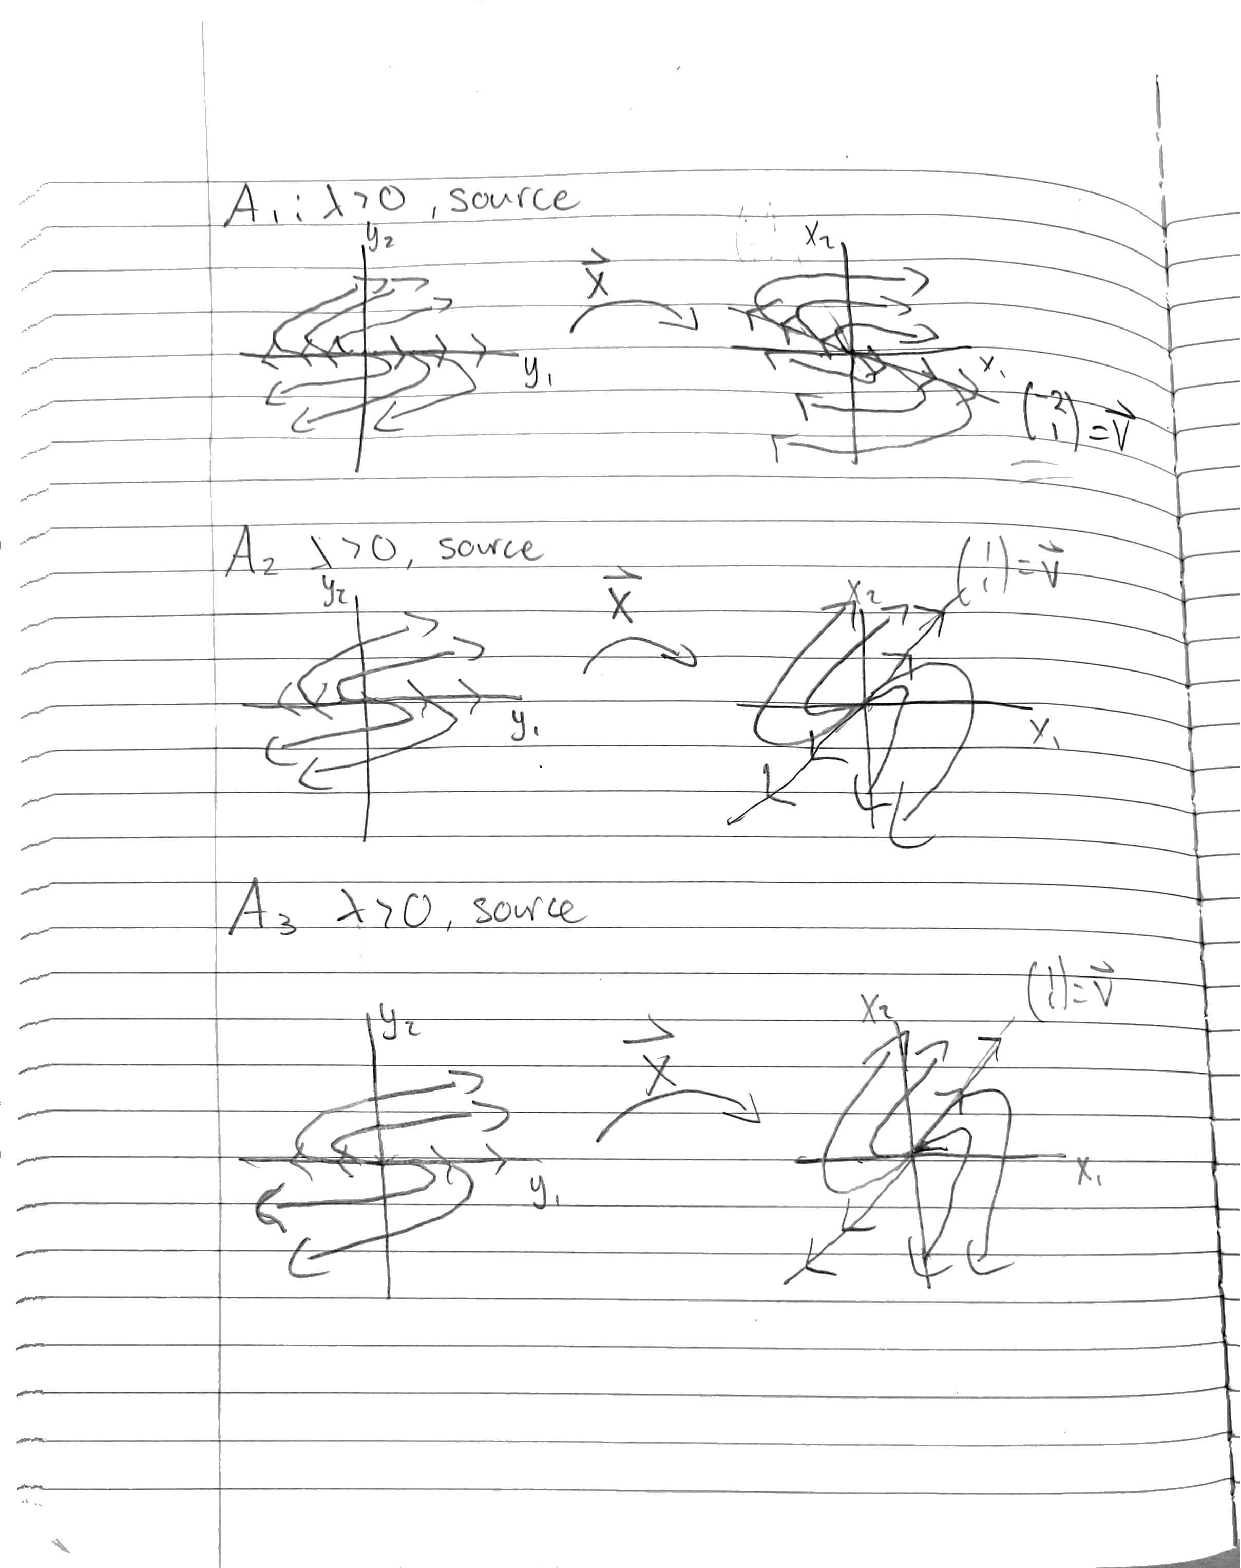
\includegraphics[width=0.6\textwidth]{PhasePlane.pdf}
            \caption{Phase Planes}
        \label{fig:phase_diagram}
    \end{figure}

    
\end{solution}

\begin{problem}{2}
    Prove that for a real \(2 \times 2\) matrix \(A\), that
    \[
        \langle A\vec{v}, \vec{w} \rangle = \langle \vec{v}, A^T\vec{w} \rangle
    \]
\end{problem}

\begin{solution}
    Let \(A = \begin{pmatrix}
        a & b \\
        c & d
    \end{pmatrix}\).
    
    Then,
    \[
        \begin{aligned}
            \langle A\vec{v}, \vec{w} \rangle &= \langle \begin{pmatrix}
                a & b \\
                c & d
            \end{pmatrix} \begin{pmatrix}
                v_1 \\
                v_2
            \end{pmatrix}, \begin{pmatrix}
                w_1 \\
                w_2
            \end{pmatrix} \rangle\\
            &= \langle \begin{pmatrix}
                av_1 + bv_2 \\
                cv_1 + dv_2
            \end{pmatrix}, \begin{pmatrix}
                w_1 \\
                w_2
            \end{pmatrix} \rangle\\
            &= (av_1 + bv_2)w_1 + (cv_1 + dv_2)w_2\\
            &= av_1w_1 + bv_2w_1 + cv_1w_2 + dv_2w_2\\
            &= aw_1v_1 + cw_2v_1 + bw_1v_2 + dw_2v_2\\
            &= (aw_1 + cw_2)v_1 + (bw_1 + dw_2)v_2\\
            &= \langle \begin{pmatrix}
                aw_1 + cw_2 \\
                bw_1 + dw_2
            \end{pmatrix}, \begin{pmatrix}
                v_1 \\
                v_2
            \end{pmatrix} \rangle\\
            &= \langle \begin{pmatrix}
                a & c \\
                b & d
            \end{pmatrix} \begin{pmatrix}
                w_1 \\
                w_2
            \end{pmatrix}, \vec{v} \rangle\\
            &= \langle A^T\vec{w}, \vec{v} \rangle
        \end{aligned}
    \]
\end{solution}

\begin{problem}{3}
    Defining \(p(\lambda) = \det(\lambda I - A)\), prove that \(\det(A^T - \lambda I) = p(\lambda)\), which is to say, the eigenvalues of a real matrix are the same as its transpose.
\end{problem}

\begin{solution}
    \textbf{Proof for \(2 \times 2\):}

    Let \(A = \begin{pmatrix}
        a & b \\
        c & d
    \end{pmatrix}\).

    Then,
    \[
        \begin{aligned}
            p(\lambda) &= \det(A - \lambda I)\\
            &= \det\begin{pmatrix}
                a - \lambda & b \\
                c & d - \lambda
            \end{pmatrix}\\
            &= (a - \lambda)(d - \lambda) - bc\\
            &= \lambda^2 - (a+d)\lambda + (ad - bc)\\
            &= \lambda^2 - \Tr(A)\lambda + \det(A)
        \end{aligned}
    \]
    Now for \(\det(A^T - \lambda I)\):
    \[
        \begin{aligned}
            \det(A^T - \lambda I) &= \det\begin{pmatrix}
                a - \lambda & c  \\
                b & d - \lambda
            \end{pmatrix}\\
            &= (a - \lambda)(d - \lambda) - cb\\
            &= \lambda^2 - (a+d)\lambda + (ad - bc)\\
            &= \lambda^2 - \Tr(A)\lambda + \det(A)\\
            &= p(\lambda)
        \end{aligned}
    \]
    Therefore, the eigenvalues of a real matrix are the same as its transpose in \(\RR^2\).

    
\end{solution}

\begin{problem}{4}
    Prove that \(A^{-1}\) exists if and only if \(A^{-T}\) exists.
\end{problem}

\begin{solution}
    Let \(A = \begin{pmatrix}
        a & b \\
        c & d
    \end{pmatrix}\) be a matrix.

    Assume \(A^{-1}\) exists.

    Then,
    \[
        A^{-1} = \frac{1}{\det(A)}\begin{pmatrix}
            d & -b \\
            -c & a
        \end{pmatrix}
    \]
    where \(\det(A) = ad - bc \neq 0\).

    Consider \(A^T = \begin{pmatrix}
        a & c \\
        b & d
    \end{pmatrix}\)
    
    \(\det(A^T) = ad - bc = \det(A) \neq 0\). So,

    \[
        A^{-T} = \frac{1}{\det(A)}\begin{pmatrix}
            d & -c \\
            -b & a
        \end{pmatrix}
    \]
    exists.


    Now, assume \(A^{-T}\) exists. Then,
    \[
        A^{-T} = \frac{1}{\det(A^T)}\begin{pmatrix}
            d & -b \\
            -c & a
        \end{pmatrix}
    \]
    So, \(A^{-1}\) exists because \(\det(A) = \det(A^T)\), and there is no division by zero.
\end{solution}

\begin{problem}{5}
    Prove that \(A^{-1}\) does not exist if 0 is an eigenvalue of \(A\).
\end{problem}

\begin{solution}
    Let 0 be an eigenvalue of \(A\). Assume, for the sake of contradiction, that \(A^{-1}\) exists.

    By definition of eigenvalue and eigenvector,
    \[
        \begin{aligned}
            A\vec{v} &= 0\vec{v} \quad \text{where } \vec{v} \neq 0\\
            A\vec{v} &= 0\\
            A^{-1}A\vec{v} &= A^{-1}0\\
            \vec{v} &= 0
        \end{aligned}
    \]
    This is a contradiction, so \(A^{-1}\) does not exist.

\end{solution}

\begin{problem}{6}
    We say for a real \(2 \times 2\) matrix \(A\) that \(\vec{b} \in \rng(A)\) if there exists \(\vec{x}\) such
    that
    \[
        A\vec{x} = \vec{b}
    \]
    Prove that \(\vec{b} \in \rng(A)\) if and only if \(\langle \vec{b}, \vec{y} \rangle = 0\) for all \(\vec{y} \in \ker(A^T)\).
    Note, for a nontrivial \(2 \times 2\) matrix, \(\ker(A^T)\) is either trivial or onedimensional. Thus either \(A^{-T}\) (and thus \(A^{-1}\)) exists, or \(b\) and any
    \(y \in \ker(A^T)\) form a basis of \(\RR^2\).
\end{problem}

\begin{solution}
    \textbf{Part 1:} Assume \(\vec{b} \in \rng(A)\).

    Then, there exists \(\vec{x}\) such that \(A\vec{x} = \vec{b}\).

    Let \(\vec{y} \in \ker(A^T)\).

    Consider \(\langle \vec{b}, \vec{y} \rangle\):
    \[
        \begin{aligned}
            \langle \vec{b}, \vec{y} \rangle &= \langle A\vec{x}, \vec{y} \rangle\\
            &= \langle \vec{x}, A^T\vec{y} \rangle\\
            &= \langle \vec{x}, 0 \rangle\\
            &= 0
        \end{aligned}
    \]
    Therefore, \(\langle \vec{b}, \vec{y} \rangle = 0\) for all \(\vec{y} \in \ker(A^T)\).

    \textbf{Part 2:} Assume \(\langle \vec{b}, \vec{y} \rangle = 0\) for all \(\vec{y} \in \ker(A^T)\).

    If \(\ker(A^T)\) is trivial, then \(\ker(A)\) is also trivial, so \(A\) spans all of \(\RR^2\), and thus \(\vec{b}\) is in the range of \(A\).

    If \(\ker(A^T)\) is not trivial, then there exists a nonzero \(\vec{y}\) such that \(A^T\vec{y} = 0\).

    \(\langle \vec{b}, \vec{y} \rangle = 0\) implies that \(\vec{b} \perp \vec{y}\).

    The Fundamental Theorem of Linear Algebra says \(\RR^2 = \rng(A) \oplus \ker(A^T)\).

    Since \(\vec{b} \perp \vec{y}\) and \(\vec{y} \in \ker(A^T)\), then \(\vec{b} \in \rng(A)\).    
\end{solution}

\begin{problem}{7}
    For real \(2 \times 2\) matrix \(A\) suppose that \(\Tr(A) = 4\det(A)\), and \(A \neq cI\), so that \(A\) has a repeated, degenerate, eigenvalue \(\lambda_0\), i.e.
    \[
        \det(A - \lambda I) = (\lambda - \lambda_0)^2\,.
    \]
    \begin{itemize}
        \item Let \(A\vec{v} = \lambda_0\vec{v}\) and suppose \(\vec{w} \cdot \vec{v} = 0\) (which we can always find
        via Gram-Schmidt). Show that
        \[
            A^T\vec{w} = \lambda_0\vec{w}
        \]
        Hint: Using the results from the prior problems, if \(A\) only has
        one eigenvalue, then so does \(A^T\). Likewise, we’re in \(\RR^2\), so two non-trivial orthogonal vectors form a basis.
        \item From this and the previous problem, show that \(\vec{v} \in \rng(A - \lambda_0I)\).
        Therefore we can find \(\vec{z}\) such that
        \[
            (A - \lambda_0I)\vec{z} = \vec{v}
        \]
        \item Show finally that
        \[
            A(\vec{v} \vec{z}) = (\vec{v} \vec{z}) \begin{pmatrix}
                \lambda_0 & 1 \\
                0 & \lambda_0
            \end{pmatrix}
        \]
        \item What ensures that \((\vec{v} \vec{z})^{-1}\) exists?
    \end{itemize}
\end{problem}

\begin{solution}
    \textbf{Part 1:}

    Let \(\lambda_0\) be the only eigenvalue of \(A\) and \(\vec{v}\) the only eigenvector of \(A\). Let \(\vec{w} \cdot \vec{v} = 0\).

    \(\vec{v} \in \ker(A - \lambda_0I)\)

    \(\vec{v} \cdot \vec{w} = 0 \implies \vec{v} \perp \vec{w}\).

    FTLA says \(\RR^2 = \ker(A - \lambda_0I) \oplus \rng(A^T - \lambda_0I)\).

    \(\vec{v} \in \ker(A^T - \lambda_0I)\ \implies \vec{w} \in \rng(A^T - \lambda_0I)\).

    \[
        \begin{aligned}
            (A - \lambda_0I)\vec{v} &= 0\\
            \langle (A - \lambda_0I)\vec{v}, \vec{w} \rangle &= 0\\
            \langle \vec{v}, (A^T - \lambda_0I)\vec{w} \rangle &= 0 \quad (*)\\
        \end{aligned}
    \]
    \(\implies \vec{v} \perp (A^T - \lambda_0I)\vec{w} \quad\) where \(\vec{v} \perp \vec{w}\)

    \(\implies (A^T - \lambda_0I)\vec{w} = c\vec{w}\)

    \(c = 0\) because of (*)

    So, \((A^T - \lambda_0I)\vec{w} = 0\)

    Then, \(\vec{w} \in \ker(A^T - \lambda_0I)\)

    Therefore, \(A^T\vec{w} = \lambda_0\vec{w}\)

    \textbf{Part 2:}

    \(\vec{w} \in \ker(A^T - \lambda_0I)\)

    FTLA says \(\RR^2 = \ker(A^T - \lambda_0I) \oplus \rng(A - \lambda_0I)\)

    \(\vec{v} \in \rng(A - \lambda_0I)\)

    Therefore, \(\exists \vec{z}\) such that \((A - \lambda_0I)\vec{z} = \vec{v}\)

    \textbf{Part 3:}

    \((A - \lambda_0I)\vec{z} = \vec{v}\)

    \(A\vec{z} = \lambda_0\vec{z} + \vec{v}\)

    \[
        \begin{aligned}
            A\vec{z} &= \lambda_0\vec{z} + \vec{v}\\
            A(\vec{v} \vec{z}) &= (\lambda_0\vec{v} \: | \: \lambda_0\vec{z} + \vec{v})\\
            &= (\vec{v} \: | \: \vec{z}) \begin{pmatrix}
                \lambda_0 & 1 \\
                0 & \lambda_0
            \end{pmatrix}
        \end{aligned}
    \]

    \textbf{Part 4:}

    \((\vec{v} \vec{z})^{-1}\) exists because \(\vec{v} \cdot \vec{z} = 0\). Two non-zero orthogonal vectors form a basis, so \((\vec{v} \vec{z})\) is invertible.
    
    

\end{solution}
    



\end{document}